% -*- mode: latex; tex-main-file: "abstract.tex" -*-
\preparagraphspacing{}
\section*{Change Descriptors}
\label{sec:chdescs}

% What they are
% What they're for, abstractly (short)
% History, better than GEOM, JBD
% How to generate the correct chdescs
% What they contain (code)
% How they move around
% How we use them (transformations, applications)
% Relationship to consistency models
% User-level chdescs
% Chdesc challenges - memory pressure, time, circularity

The ability to revert and re-apply change descriptors is inspired by the soft
updates system in BSD's FFS~\cite{ganger00soft}, but it is generalized so that
it is not specific to any particular filesystem. A simplified version of the
change descriptor structure is shown in Figure~\ref{fig:chdesc}.

\begin{figure}
\begin{verbatim}
struct chdesc {
    BD_t *owner;
    bdesc_t *block;
    enum {BIT, BYTE, NOOP} type;
    union {
        struct {
            uint16_t offset;
            uint32_t xor;
        } bit;
        struct {
            uint16_t offset, length;
            uint8_t *data;
        } byte;
    };
    struct chdesc *dependencies[];
};
\end{verbatim}
\vspace{-12pt}
\caption{\label{fig:chdesc} Change descriptor structure}
\end{figure}

When a KudOS module first generates change descriptors in order to write changes
to the disk, it connects them together to express its write ordering
requirements. Then it passes the change descriptors to another module in the
direction of the disk, which can then inspect and even modify them before
passing them on. Soft updates, journalling, and many application-specific
consistency models all correspond to different change descriptor arrangements,
so these features can be added to the system (and to any filesystem) as modules
which appropriately connect or reconnect the change descriptors.

For example, we have implemented journalling as a single block device module, to
which any filesystem module can be attached. Even metadata-only journalling is
possible with this design, though our module does not yet have this feature.
Other block device layering systems, like GEOM~\cite{geom} or JBD in Linux,
would or do need special hooks into filesystem code in order to get the
necessary hints (i.e. what is metadata and what is not) to do metadata-only
journalling. Change descriptors (and the LFS interface division described in the
next section) allow us to do this automatically.

\begin{figure}[b]
  \centering
  \includegraphics[width=80pt]{fig/whatevs_3}
  \caption{\label{fig:softupdates} Soft updates change descriptor graph.}{These
  change descriptors represent the dependencies for adding a newly allocated
  block to an inode. Writing the new block pointer to an inode ($BP$) depends
  on initializing the block ($ZB$) and updating the free block map ($AB$).
  Updating the size of the inode ($US$) depends on writing the block pointer
  ($BP$).
}
\end{figure}

\begin{figure}
  \centering
  \includegraphics[width=200pt]{fig/whatevs_2}
  \caption{\label{fig:journal} Journal change descriptor graph.}{The original
  four change descriptors from Figure~\ref{fig:softupdates} are made to depend
  on a journal commit record, which depends on copies ($ZB_j$, $AB_j$, $BP_j$,
  and $US_j$) of the original change descriptors being written to the journal. A
  commit record cancellation depends on the original change descriptors. The
  empty circles are ``NOOP'' change descriptors which have no associated block
  data.
}
\end{figure}

For many complex operations, like RAID or journalling, the chdesc graph is
changed in specific ways which can be broken down into sequences of simple graph
transformations. For example, in the (mirroring) RAID module it is necessary to
duplicate a change descriptor, including all its dependents and dependencies. We
expect that after implementing a relatively small number of more complex modules
(we have only implemented the two mentioned), we will have seen similarities in
many of the transformations and will have built up a fairly complete library of
common transformation functions.

\begin{figure}
  \centering
  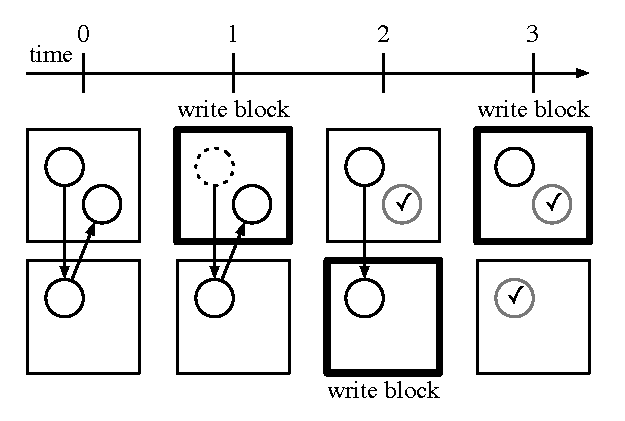
\includegraphics[width=200pt]{rollback_sequence}
  \caption{\label{fig:rollback} Rolling back change descriptors.}{Although no
  cycles are allowed in change descriptor graphs, cycles can exist at the block
  level which require some change descriptors to be rolled back in order to
  write the blocks. Here the squares are blocks, and dotted circles are rolled
  back change descriptors.
}
\end{figure}
